\subsection{Leistungsverhalten bei Spannungsabfall}\label{subsec:LeistungSpannungabfall}
Bei diesem Versuch wird das Verhalten des Controllers bei einem Spannungsabfall untersucht. Dabei wird sowohl die Leistung der ASM (Abbildung \ref{fig:Spannungsabfall} rechts) als auch der Strom des Controllers (Abbildung \ref{fig:Spannungsabfall} links) in Abhängigkeit zur Spannung des Controllers gemessen. Der Drehmoment-Sollwert wird während des gesamten Versuchs konstant auf dem Nennmoment gehalten. Die Versuchsbedingungen sind in der Tabelle \ref{tab:Spannungsabfall} enthalten.

\begin{table}[H]
	\centering
	\begin{tabular}{C{4cm} C{4cm} C{3cm}} 
		\multicolumn{3}{c}{\textbf{Versuchsbedingungen}} \\
		{Messgrösse}& {Bedingung} & {Wert}\\ \hline\hline 
		Spannung (DC)   & variiert &   72-103 V     \\
		Strom (DC)   & gemessen &   68.7-124 A     \\
		Leistung (AC)   & gemessen &   4420-6420 W    \\
		Drehzahl   & variiert &   1500/2000 RPM    \\
		Drehmoment-Sollwert   & konstant &   32 Nm    \\
		Motor-Temperatur   & gemessen &   30-90 °C    \\
		Controller-Temperatur   & vernachlässigt &   -    \\
	\end{tabular}
	\caption{Versuchsbedingungen Spannungsabfall}\label{tab:Spannungsabfall}
\end{table}


In Abbildung \ref{fig:Spannungsabfall} sind die Messwerte des Versuchs abgebildet. Zuerst ist der Versuch mit 2000 RPM (blaue Punkte) und danach nochmals mit 1500 RPM (rote Punkte) durchgeführt worden. Wird die Leistungs-Temperaturabhängigkeit berücksichtigt (schwarze und rosa Punkte), dann ist ersichtlich, dass die Leistung nicht von der Spannung, sondern lediglich von der Temperatur abhängig ist.

\begin{figure}[H]
	\centering
	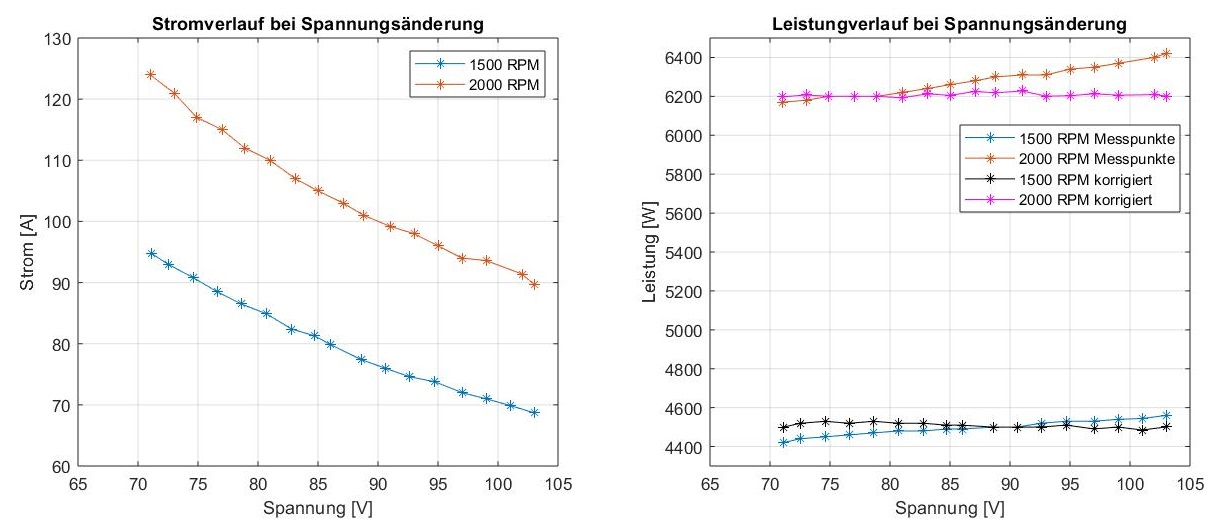
\includegraphics[width=1\linewidth]{Spannungsversuch.jpg}
	\caption{Leistungs- und Stromverlauf bei Spannungsabfall}\label{fig:Spannungsabfall}
\end{figure}

Da die Leistung unabhängig von der Versorgungsspannung ist, solange diese über einem bestimmten Grenzwert liegt (Unterkapitel \ref{subsec:LeistungSpannungsabfall} und \ref{subsec:DrehzahlSpanungsabfall}), muss diese bei der Kraftregelung nicht berücksichtigt werden.